\documentclass[11pt,a4paper]{article}

% --- Encoding & Fonts ---
\usepackage[T1]{fontenc}
\usepackage[utf8]{inputenc}

% --- Table Formatting ---
\usepackage{tabularx}
\usepackage{tabularx}
\usepackage{ragged2e}
\usepackage{booktabs}

% --- Math Packages ---
\usepackage{amsmath,amssymb,amsthm}

% --- Layout & Graphics ---
\usepackage[margin=1in]{geometry}
\usepackage{parskip}
\usepackage{xcolor}
\usepackage{booktabs}
\usepackage{hyperref}

% --- Code Listings Configuration ---
\usepackage{tikz}
\usetikzlibrary{positioning}
\usepackage{forest}
\usepackage{listings}
\lstset{
  basicstyle=\small\ttfamily,
  breaklines=true,
  frame=single,
  backgroundcolor=\color{gray!5},
  keywordstyle=\color{blue},
  commentstyle=\color{green!50!black},
  stringstyle=\color{orange},
  showstringspaces=false,
  language=Python,
  literate={≥}{{$\geq$}}1 {→}{{$\to$}}1 {τ}{{$\tau$}}1 {𝓐}{{$\mathcal{A}$}}1 {⟨}{{$\langle$}}1 {⟩}{{$\rangle$}}1
}

% --- Environment Definitions ---
\newtheorem{definition}{Definition}
\newtheorem{principle}{Principle}

% ==========================================================
% Title & Author Information
% ==========================================================
\title{\textbf{Anchor Architecture: \\ A Minimal Structural Foundation for Software Traceability}}

\author{
  Spark Tsai \\
  ORCID: \href{https://orcid.org/0009-0006-8847-4703}{0009-0006-8847-4703} \\
  Email: \href{mailto:spark.tsai@gmail.com}{spark.tsai@gmail.com}
}
\date{February 2026}

\begin{document}
\maketitle

% ==========================================================
% Abstract
% ==========================================================
\begin{abstract}
As software development increasingly incorporates AI assistance and autonomous agents, the structural relationships between specifications, code, tests, and governance artifacts often degrade into post-hoc reconstruction. Existing traceability approaches share a common assumption: that entities are already structurally identifiable. When identifiers, locations, and temporal states are not bound to artifacts at creation time, subsequent analysis becomes speculative. 

This paper presents \textbf{Anchor Architecture}, a model-independent, pre-analytical framework that defines the structural conditions under which traceability becomes deterministic. The framework consists of exactly two primitives: the \textbf{Anchor}, a spatiotemporal coordinate $\langle ID, L, \tau \rangle$, and the \textbf{Relationship}, a directed binary relation $R \subseteq \mathcal{A} \times \mathcal{A}$. From these, four structural views (\textit{Linear, Net, Set, Timeline}) and four operations (\textit{trace, impact, diff, version}) are derived, grounded in relation theory and set theory. 

The central claim is that traceability failures stem from missing structural anchors rather than opaque reasoning. We formalize pre-analytical anchoring as a necessary condition for structural examinability. By reducing traceability to a problem of coordinate geometry, the architecture enables deterministic impact analysis and integrity validation, providing a mathematical safeguard against AI hallucinations in engineering governance—independent of specific AI models, tooling, or semantic interpretation.
\end{abstract}

% ==========================================================
% Keywords Section
% ==========================================================
\textbf{Keywords:} Anchor Architecture, Structural Traceability, Spatiotemporal Coordinate, Pre-Analytical Anchoring, Relation Theory, Software Engineering, AI-Assisted Development

% ==========================================================
% Section 1: Introduction
% ==========================================================
\section{Introduction}
Software artifacts — specifications, code, tests, configurations — are increasingly produced through hybrid authorship involving human developers and AI agents [6][8]. Regardless of the author, a recurring structural problem persists: relationships between artifacts are reconstructed after the fact. Provenance models [1] assume entities are already identifiable; version control tracks file-level states but not arbitrary structural entities; traceability matrices [2] collapse under annotation overhead; supply chain frameworks [4][5] presuppose well-defined artifact boundaries. None address the foundational question: what minimal structural condition must hold *before* any traceability mechanism can operate?

This paper argues that traceability failures are caused by \textbf{missing structural anchors} — not by opaque reasoning, insufficient documentation, or inadequate tooling. When identifiers, locations, and temporal states are not bound to artifacts at creation time, all subsequent analysis becomes reconstructive and therefore speculative. This condition is non-reconstructible: structure absent at creation cannot be recovered with certainty post-hoc.

To address this, the paper presents \textbf{Anchor Architecture}, a minimal, model-independent framework consisting of exactly two primitives: \textbf{Anchor}, a spatiotemporal coordinate $\langle ID, L, \tau \rangle$ that binds identity to a persistent location and temporal index; and \textbf{Relationship}, a directed binary relation $R \subseteq \mathcal{A} \times \mathcal{A}$ over the anchor set. From these primitives, the framework derives four structural views — Linear, Net, Set, and Timeline — as projections over the relational structure $(\mathcal{A}, R)$, and four operations — trace(), impact(), diff(), version() — as compositions over the primitive relation, without additional axioms.

The contributions of this paper are: (1) a minimal primitive foundation grounded in relation theory and set theory; (2) derived structural views and operations that reduce failure diagnosis, impact analysis, change detection, and integrity validation to coordinate operations; and (3) a formal characterization of pre-analytical anchoring as a necessary condition for structural examinability. A comprehensive worked example demonstrating these operations over a concrete development scenario is provided in Appendix.

% ==========================================================
% Section 2: Anchor
% ==========================================================
\section{Anchor}
An \textbf{Anchor} is a spatiotemporal coordinate that binds identity to a persistent location and a temporal state. An anchor does not contain content. It defines where and when content exists.

% ==========================================================
% Section 2.1: Definition
% ==========================================================
\subsection{Definition}

% ==========================================================
% Section 2.1.1: Identifier (ID)
% ==========================================================
\subsubsection{Identifier (ID)}
An \textbf{Identifier (ID)} establishes a persistent logical reference to a structural entity.

Formally:
\begin{equation}
ID = f_{id}(Entity)
\end{equation}

A \textbf{Structural Entity} is independently referenceable:
\begin{itemize}
    \item Requirement paragraph
    \item Function
    \item Test
    \item Transaction
\end{itemize}

Properties:
\begin{itemize}
    \item Entity Naming
    \item Location Neutral
    \item Temporal Neutral
    \item Structural Necessity
\end{itemize}

% ==========================================================
% Section 2.1.2: Spatial Anchor
% ==========================================================
\subsubsection{Spatial Anchor}
A Spatial Anchor binds identity to a persistent location.

\begin{equation}
A_s = \langle ID, L \rangle
\end{equation}

Locator must satisfy \textbf{Resolvability}:
\begin{equation}
resolve(\langle ID, L \rangle) \to Content
\end{equation}

% ==========================================================
% Section 2.1.3: Spatiotemporal Anchor
% ==========================================================
\subsubsection{Spatiotemporal Anchor}
A \textbf{Spatiotemporal Anchor} binds identity, location, and time into a single structural primitive. It is formally expressed as:

\begin{equation}
\mathcal{A} = \langle ID, L, \tau \rangle
\end{equation}

where $\tau$ is a temporal index that establishes when the anchor state was committed.

Version identifiers are not the only admissible representation.
Any value that resolves to a deterministic temporal position is valid: \texttt{v1.2}, \texttt{a3f7c2d}, \texttt{2026-02-15T10:30:00Z}.

\begin{equation}
    \tau = v1.2 \;\mapsto\; \text{commit } \texttt{a3f7c2d} \;\mapsto\; \text{2026-02-15T10:30:00Z}
\end{equation}

The requirement is not a specific format, but \textbf{resolvability to a unique temporal position}. 
All representations that satisfy this condition are structurally equivalent as $\tau$.

% ==========================================================
% Section 2.2: Coordinate Structure
% ==========================================================
\subsection{Coordinate Structure}

\noindent Anchoring proceeds as monotonic expansion:

\begin{equation}
ID \rightarrow \langle ID, L \rangle \rightarrow \langle ID, L, \tau \rangle
\end{equation}

Each expansion increases structural determinacy:

\begin{table}[h]
\centering
\renewcommand{\arraystretch}{1.5}
\begin{tabular}{lll}
\hline
\textbf{Coordinate} & \textbf{Establishes} & \textbf{Enables} \\ \hline
$ID$ & Existence & Identity reference \\
$\langle ID, L \rangle$ & Resolvability & Deterministic resolution \\
$\langle ID, L, \tau \rangle$ & Examinability & Historical query, temporal comparison \\ \hline
\end{tabular}
\end{table}

\noindent Identity is separated from state. \\
The same $ID$ at the same $L$ may exist at multiple $\tau$, and each $\langle ID, L, \tau \rangle$ is a distinct coordinate.

% ==========================================================
% Section 2.3: Structural Properties
% ==========================================================
\subsection{Structural Properties}
Two anchors are identical if and only if all coordinate components match.

\medskip
\noindent \textbf{Spatial identity:}

\begin{equation}
\langle ID, L \rangle = \langle ID', L' \rangle \iff ID = ID' \land L = L'
\end{equation}

\noindent \textbf{Spatiotemporal identity:}

\begin{equation}
A = A' \iff ID = ID' \land L = L' \land \tau = \tau'
\end{equation}

Consequently, the same $ID$ at the same $L$ with different $\tau$ yields distinct anchors --- this is what makes versioning \textit{structurally expressible} rather than \textit{conventionally imposed}.

% ==========================================================
% Section 2.4: Existence and Determinacy
% ==========================================================
\subsection{Existence and Determinacy}

Anchors must be committed at creation time.
If an anchor does not exist prior to analysis,
all subsequent analysis becomes speculative.

\medskip
\noindent This condition is non-reconstructible:
multiple histories can produce identical present states.
A temporal index not recorded at creation
cannot be uniquely recovered post-hoc.

\begin{equation}
\neg \exists\, \tau_{\text{created}} \;\Rightarrow\; \neg \exists\, \text{unique reconstruction of } \tau
\end{equation}

\noindent Pre-analytical anchoring is therefore a necessary condition
for structural examinability --- not a best practice,
but a prerequisite.

% ==========================================================
% Section 3: Relationship
% ==========================================================
\section{Relationship}

% ==========================================================
% Section 3.1: Definition
% ==========================================================
\subsection{Definition}
A \textbf{Relationship} is a binary relation over the set of anchors $\mathcal{A}$:
\begin{equation}
R \subseteq \mathcal{A} \times \mathcal{A}
\end{equation}

An instance of relationship is an ordered pair:
\begin{equation}
(a_i, a_j) \in R
\end{equation}

It expresses \textbf{structural adjacency only}.  \\
No embedded semantics are carried at the architectural layer. \\
Terms such as \textit{implements}, \textit{tests}, \textit{validates}, \textit{depends-on}, or \textit{governs} are not primitives of the architecture. \\
They are interpretations applied externally by domain-specific rules. \\
The architecture is defined entirely in relational terms. \\
No additional structural primitives are required. 

% ==========================================================
% Section 3.2: Validity
% ==========================================================
\subsection{Validity}

A relationship is structurally valid if and only if both participating anchors are resolvable:

\begin{equation}
(a_i, a_j) \in R_{\text{valid}}
\iff
\operatorname{resolve}(a_i) \neq \varnothing
\land
\operatorname{resolve}(a_j) \neq \varnothing
\end{equation}

\noindent Validity is therefore determined by coordinate existence, not symbolic declaration.

\medskip
\noindent If 

\begin{equation}
\operatorname{resolve}(a_i) = \varnothing
\end{equation}

\noindent then no valid relationship involving $a_i$ can exist.

\medskip
\noindent Structural validity is binary. It is not inferred, repaired, or interpreted. It is decided by resolvability.

% ==========================================================
% Section 3.3: Closure and Reachability
% ==========================================================
\subsection{Closure and Reachability}

Define the transitive closure:

\begin{equation}
R^{+} = \bigcup_{n=1}^{\infty} R^n
\end{equation}

where $R^1 = R$ and $R^{n+1} = \{(a_i, a_k) \mid \exists\, a_j : (a_i, a_j) \in R^n \land (a_j, a_k) \in R\}$.

\medskip
\noindent Traceability is reachability over $R^{+}$. 
Impact analysis, dependency chains, and evidence paths reduce to membership queries in $R^{+}$.

\medskip
\noindent Reachability is determined by declared relations, not temporal ordering.
Given $(a_1, a_2) \in R$, temporal consistency may require:

\begin{equation}
\tau_1 \le \tau_2
\end{equation}

\noindent But temporal precedence alone does not generate relation:

\begin{equation}
\tau_1 < \tau_2 \;\not\Rightarrow\; (a_1, a_2) \in R
\end{equation}

\noindent Time constrains admissible direction; relation must be declared independently.
If $(a_1, a_2) \in R \land \tau_1 > \tau_2$, 
the relation is temporally inconsistent --- a structural violation detectable through coordinate comparison, not semantic inspection.

% ==========================================================
% Section 3.4: Structural Constraints
% ==========================================================
\subsection{Structural Constraints}

The relation $R$ is intentionally minimally constrained:

\begin{equation}
\begin{aligned}
&(a_1, a_2) \in R \land (a_1, a_3) \in R &&\text{is permitted (not a function)} \\
&(a_1, a_2) \in R \nRightarrow (a_2, a_1) \in R &&\text{(not symmetric)} \\
&(a_1, a_2) \in R \land (a_2, a_3) \in R \nRightarrow (a_1, a_3) \in R &&\text{(not transitive)} \\
\end{aligned}
\end{equation}

\noindent No cardinality, hierarchy, acyclicity, or reflexivity constraints are imposed.

\medskip
\noindent \textbf{Semantic neutrality.} \\
Relationship types such as \textit{implements}, \textit{tests}, \textit{governs}, or \textit{constrains} are not architectural primitives. 
They are application-layer interpretations imposed over structural adjacency. 
The relation is invariant; meaning is delegated.

\medskip
\noindent \textbf{Temporal independence.} \\
Temporal precedence does not generate relation:

\begin{equation}
\tau(a_i) < \tau(a_j) \;\not\Rightarrow\; (a_i, a_j) \in R
\end{equation}

\noindent Relation must be declared independently. 
Application-layer policies may optionally impose $\tau(a_i) \le \tau(a_j)$ to enforce causal or lifecycle consistency, 
but such constraints are governance-layer rules, not structural necessities.

% ==========================================================
% Section 4: Relational Views
% ==========================================================
\section{Relational Views}
Structural views are derived subrelations of the global relation $R$.

% ==========================================================
% Section 4.1: Formal Definition
% ==========================================================
\subsection{Formal Definition}
The global relation is defined as:
\begin{equation}
R \subseteq \mathcal{A} \times \mathcal{A}
\end{equation}

A structural view is defined by a predicate $C$:
\begin{equation}
R_{\text{view}} = \{ (a_i, a_j) \in R \mid C(a_i, a_j) \}
\end{equation}

Thus:
\begin{equation}
R_{\text{view}} \subseteq R
\end{equation}

Structural views introduce no new primitives. \\
They operate over the same anchor set $\mathcal{A}$ and relation set $R$. \\
No structural elements are added or modified.

% ==========================================================
% Section 4.2: View Categories (Predicate Families)
% ==========================================================
\subsection{View Categories (Predicate Families)}
Different engineering concerns correspond to different predicates. \\
The following view categories are illustrative, not exhaustive. \\
Any predicate over anchors or their coordinates may define a valid structural view.

% ==========================================================
% Section 4.2.1: Causal View
% ==========================================================
\subsubsection{Causal View}

Define the causal subrelation of $R$ as:

\begin{equation}
R_{causal} = \{ (a_i, a_j) \in R \mid \tau(a_i) \le \tau(a_j) \}
\end{equation}

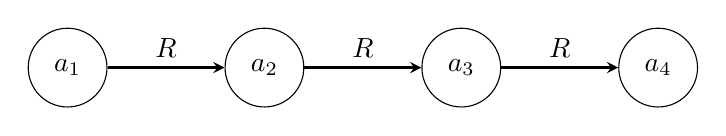
\begin{tikzpicture}[>=stealth, node distance=2.5cm]
  \node[draw, circle, minimum size=1cm] (A1) {$a_1$};
  \node[draw, circle, minimum size=1cm, right of=A1] (A2) {$a_2$};
  \node[draw, circle, minimum size=1cm, right of=A2] (A3) {$a_3$};
  \node[draw, circle, minimum size=1cm, right of=A3] (A4) {$a_4$};
  \draw[->, thick] (A1) -- node[above] {$R$} (A2);
  \draw[->, thick] (A2) -- node[above] {$R$} (A3);
  \draw[->, thick] (A3) -- node[above] {$R$} (A4);
\end{tikzpicture}

\noindent This is a derived subrelation obtained by restricting $R$ under temporal monotonicity.

\medskip
\noindent Causal View does not modify $R$. It filters $R$ according to a temporal predicate.

\medskip
\noindent Backward references may remain structurally valid in $R$, but are excluded from causal analysis.

% ==========================================================
% Section 6.2.2: Cross-Artifact View
% ==========================================================
\subsubsection{Cross-Artifact View}

\begin{equation}
C_{cross}(a_i, a_j) \iff L_{a_i} \neq L_{a_j}
\end{equation}

This isolates inter-artifact relationships.

\textbf{Example}

Given anchors:
\begin{align*}
A_1 &= \langle \text{FR-091, srs/auth.md, v1.2} \rangle \\
A_2 &= \langle \text{FR-095, srs/auth.md, v1.2} \rangle
\end{align*}

\begin{verbatim}
---
location: srs/auth.md
version: v1.2
---

### FR-091
Password length must be >= 12 characters.

### FR-095
Passwords must be stored using a secure hashing algorithm.
\end{verbatim}

\begin{align*}
A_3 &= \langle \text{FUNC-validate, src/auth.py, v2.1} \rangle \\
A_4 &= \langle \text{TEST-length-too-short, tests/auth.py, v1.1} \rangle \\
A_5 &= \langle \text{TEST-length-eligible, tests/auth.py, v1.1} \rangle
\end{align*}

\begin{verbatim}
# file: tests/auth.py
# version: v1.1

# ID: TEST-length-too-short
# TRACE: STS-091
def test_length_too_short():

# ID: TEST-eligible
# TRACE: STS-091
def test_length_eligible():
\end{verbatim}

And relations:
\begin{equation}
R = \{ (A_1, A_2), (A_1, A_3), (A_3, A_4), (A_4, A_5) \}
\end{equation}

Cross-Artifact View filtering:
\begin{itemize}
    \item $(A_1, A_2) \notin C_{cross}$ because both in \texttt{srs/auth.md} \texttimes
    \item $(A_1, A_3) \in C_{cross}$ because \texttt{srs/auth.md} $\neq$ \texttt{src/auth.py} \checkmark
    \item $(A_3, A_4) \in C_{cross}$ because \texttt{src/auth.py} $\neq$ \texttt{tests/auth.py} \checkmark
    \item $(A_4, A_5) \notin C_{cross}$ because both in \texttt{tests/auth.py} \texttimes
\end{itemize}

\textbf{Interpretation}

Included relations (cross-artifact):
\begin{itemize}
    \item Requirement $\to$ Implementation
    \item Implementation $\to$ Test
\end{itemize}

Excluded relations (intra-artifact):
\begin{itemize}
    \item Requirement $\to$ Requirement (specification refinement)
    \item Test $\to$ Test (test case dependency)
\end{itemize}

This view isolates structural dependencies that cross artifact boundaries, useful for 
\begin{itemize}
    \item Requirement traceability to implementation
    \item Cross-repository impact analysis
    \item Governance boundary verification
\end{itemize}

% ==========================================================
% Section 6.2.3: Identity Consistency View
% ==========================================================
\subsubsection{Identity Consistency View}

\begin{equation}
C_{id}(a_i, a_j) \iff ID_{a_i} = ID_{a_j}
\end{equation}

This traces evolution of a logical component across location or time. \\
ID equality does not imply coordinate equality.

\textbf{Example}

Given anchors representing a refactored function:
\begin{align*}
A_1 &= \langle \text{FUNC-validate, src/auth.py, v1.0} \rangle \\
A_2 &= \langle \text{FUNC-validate, src/auth.py, v2.0} \rangle \\
A_3 &= \langle \text{FUNC-validate, src/utils/validation.py, v3.0} \rangle \\
A_4 &= \langle \text{UTILS-hash, src/hash.py, v1.0} \rangle
\end{align*}

\begin{verbatim}
# file: src/hash.py
# version: v1.0

# ID: UTILS-hash
# TRACE: FR-095@v1.2, STS-091@v1.0
def hash_password(password: str) -> str:
\end{verbatim}

And relations:
\begin{equation}
R = \{ (A_1, A_2), (A_2, A_3), (A_2, A_4) \}
\end{equation}

Identity Consistency View filtering:
\begin{itemize}
    \item $(A_1, A_2) \in C_{id}$ because $\text{FUNC-validate} = \text{FUNC-validate}$ \checkmark
    \item $(A_2, A_3) \in C_{id}$ because $\text{FUNC-validate} = \text{FUNC-validate}$ \checkmark
    \item $(A_2, A_4) \notin C_{id}$ because $\text{FUNC-validate} \neq \text{UTILS-hash}$ \texttimes
\end{itemize}

\textbf{Interpretation}

Included relations trace the evolution of FUNC-validate:
\begin{itemize}
    \item $A_1 \to A_2$: Same location, version upgrade
    \item $A_2 \to A_3$: Location changed (refactored to utils/), ID persists
\end{itemize}

Excluded relation crosses component boundaries:
\begin{itemize}
    \item $A_2 \to A_4$: Different logical components (validation vs hashing)
\end{itemize}

This view reveals logical continuity across refactoring, where the same component migrates between files.

\textbf{Contrast with Timeline View}
Timeline View:
\begin{equation}
Timeline(\text{FUNC-validate, src/auth.py}) = [A_1, A_2]
\end{equation}

Timeline excludes $A_3$ because location changed. \\
Identity Consistency includes $A_3$ because ID persists.

\textbf{Relationship to Other Views}

Identity Consistency View:
\begin{itemize}
    \item Requires: Same ID only
    \item Tracks: Logical component across migrations
    \item Use case: Refactoring traceability
\end{itemize}

Timeline View:
\begin{itemize}
    \item Requires: Same ID AND same location
    \item Tracks: Temporal evolution at fixed location
    \item Use case: Version history of a file
\end{itemize}

Both views operate on the same $R$. \\
The difference is constraint strictness.

% ==========================================================
% Section 6.3: Structural Forms (Induced Structures)
% ==========================================================
\subsection{Structural Forms (Induced Structures)}
Structural forms describe the geometric patterns that emerge from particular predicate-restricted subrelations. \\
They do not introduce new primitives. They characterize the shape of derived subrelations under specific constraints. \\
These forms describe recurring geometric patterns observed in predicate-restricted subrelations. Other forms may arise under different predicates.

% ==========================================================
% Section 6.3.1: Linear View
% ==========================================================
\subsubsection{Linear View}
A Linear View is a total ordered path derived from $R$.

Formally, a linear chain is a sequence of anchors:
\begin{equation}
L = [A_1, A_2, \dots, A_n]
\end{equation}

such that:
\begin{equation}
(A_i, A_{i+1}) \in R \quad \text{for all } i \in [1, n-1]
\end{equation}

In valid causal chains, temporal ordering typically follows:
\begin{equation}
\tau_1 < \tau_2 < \dots < \tau_n
\end{equation}

This represents sequential structural progression.

\textbf{Example}

Given anchors:
\begin{align*}
A_{req} &= \langle \text{FR-091, srs/auth.md, v1.2} \rangle \\
A_{sts} &= \langle \text{STS-091, sts/auth-status.md, v1.0} \rangle
\end{align*}

\begin{verbatim}
<!-- sts/auth-status.md -->
<!-- version: v1.0 -->

### STS-091
Password validation strategy defined.
\end{verbatim}

\begin{align*}
A_{code} &= \langle \text{FUNC-validate, src/auth.py, v2.1} \rangle \\
A_{log} &= \langle \text{TEST-LOG-auth, logs/test-auth.log, 2026-02-15T10:30:00Z} \rangle
\end{align*}

\begin{verbatim}
// Test Execution Log
// ID: TEST-LOG-auth
// File: logs/test-auth.log
// Timestamp: 2026-02-15T10:30:00Z⟩
{
  "test": "test_password_length",
  "result": "pass"
}
\end{verbatim}

And relations:
\begin{equation}
R = \{ (A_{req}, A_{sts}), (A_{sts}, A_{code}), (A_{code}, A_{log}) \}
\end{equation}

Then:
\begin{equation}
L = [A_{req}, A_{sts}, A_{code}, A_{log}]
\end{equation}

forms a linear chain representing the trace from:
\begin{itemize}
    \item Requirement specification
    \item Status/design document
    \item Implementation
    \item Test execution log
\end{itemize}

\textbf{Cross-Domain Traceability}

This chain spans multiple artifact types and uses mixed temporal representations (versions for documents/code, timestamp for execution logs). All are valid temporal indices in the architecture. \\
This linear chain demonstrates that Anchor Architecture supports heterogeneous artifacts without requiring schema alignment. Each anchor maintains its own temporal semantics while participating in the same structural relation.

% ==========================================================
% Section 6.3.2: Net View
% ==========================================================
\subsubsection{Net View}
The Net View represents the complete relation $R$ without additional constraints.

\begin{equation}
Net = R
\end{equation}

Characteristics:
\begin{itemize}
    \item Arbitrary branching permitted
    \item Many-to-many relational structure permitted
    \item No hierarchy enforced
    \item No tree constraint imposed
    \item No cardinality restriction
\end{itemize}

The Net View is the unfiltered relational substrate.

\textbf{Example}

Given anchors:
\begin{align*}
A_{req} &= \langle \text{FR-091, srs/auth.md, v1.2} \rangle \\
A_{sts1} &= \langle \text{STS-091, sts/length-validation.md, v1.0} \rangle \\
A_{sts2} &= \langle \text{STS-095, sts/hash-policy.md, v1.0} \rangle \\
A_{code1} &= \langle \text{FUNC-validate, src/auth.py, v2.1} \rangle \\
A_{code2} &= \langle \text{Utils-hash, src/utils/hash.py, v1.3} \rangle \\
A_{log} &= \langle \text{TEST-LOG, logs/test-auth.log, 2026-02-15T14:00:00Z} \rangle
\end{align*}

And relations:
\begin{equation}
R = \{ 
  (A_{req}, A_{sts1}), 
  (A_{req}, A_{sts2}), 
  (A_{sts1}, A_{code1}), 
  (A_{sts2}, A_{code2}),
  (A_{code1}, A_{log}),
  (A_{code2}, A_{log})
\}
\end{equation}

Relational structure:
\begin{verbatim}
              FR-091
             /      \
        STS-091    STS-095
         (Length)   (Hash)
      FUNC-validate Utils-hash
            \        /
            TEST-LOG
\end{verbatim}

This demonstrates:
\begin{itemize}
    \item \textbf{First-level branching}: One requirement decomposes into two design aspects
    \item \textbf{Parallel implementation}: Each design aspect maps to distinct code modules
    \item \textbf{Convergence}: Both implementations contribute to unified test evidence
    \item \textbf{Multi-domain trace}: From specification $\to$ design $\to$ code $\to$ execution
\end{itemize}

Net View captures the complete structural adjacency space, enabling full impact propagation and dependency analysis.

\textbf{Structural Analysis}

Forward impact from FR-091:
\begin{equation}
impact(A_{req}) = \{ A_{sts1}, A_{sts2}, A_{code1}, A_{code2}, A_{log} \}
\end{equation}

Backward trace from TEST-LOG:
\begin{equation}
trace^{-1}(A_{log}) = \{ A_{code1}, A_{code2}, A_{sts1}, A_{sts2}, A_{req} \}
\end{equation}

Both queries operate over the same relational foundation.

% ==========================================================
% Section 6.3.3: Set View
% ==========================================================
\subsubsection{Set View}
A \textbf{Set View} is a membership-based selection over anchors.

Formally:
\begin{equation}
S \subseteq \mathcal{A}
\end{equation}

Membership is defined as:
\begin{equation}
a \in S
\end{equation}

A Set View introduces \textbf{no structural relations}. It does not modify $R$. It does not imply adjacency, causality, or reachability.

Set membership is independent of:
\begin{equation}
(a_i, a_j) \in R
\end{equation}

That is:
\begin{equation}
a_i \in S \land a_j \in S \nRightarrow (a_i, a_j) \in R
\end{equation}

A Set View restricts analysis to a subset of anchors. It is a projection over $\mathcal{A}$, not a transformation of $R$.

\textbf{Example}

Define a compliance boundary for authentication subsystem:
\begin{equation}
S_{\text{auth-boundary}} = \{ 
  a \in \mathcal{A} \mid L_a \in \{\text{srs/auth.md}, \text{sts/auth.md}, \text{src/auth.py}, \text{tests/auth.py}\}
\}
\end{equation}

Given complete anchor set:
\begin{equation}
\mathcal{A} = \{
  \langle \text{FR-091, srs/auth.md, v1.2} \rangle,
  \dots,
  \langle \text{LOG-deploy, logs/deploy.log, 2026-02-15T10:00:00Z} \rangle
\}
\end{equation}

Set View result:
\begin{equation}
S_{\text{auth-boundary}} = \{
  \langle \text{FR-091, srs/auth.md, v1.2} \rangle,
  \dots,
  \langle \text{TEST-auth, tests/auth.py, v1.1} \rangle
\}
\end{equation}

Excluded anchors:
\begin{itemize}
    \item UTILS-hash (src/hash.py) --- outside auth boundary
    \item LOG-deploy (logs/deploy.log) --- deployment artifact, not auth subsystem
\end{itemize}

\textbf{Structural Independence}

Even if relations exist:
\begin{equation}
R = \{ 
  (\text{FR-091}, \text{FUNC-validate}),
  \dots,
  (\text{UTILS-hash}, \text{TEST-auth})
\}
\end{equation}

The relation $(\text{FUNC-validate}, \text{UTILS-hash}) \in R$ crosses the boundary. \\
Set View only defines membership.

% ==========================================================
% Section 6.3.4: Timeline View
% ==========================================================
\subsubsection{Timeline View}
Timeline is a constrained projection of $R$ over identical identity and location.

Given anchors:
\begin{align}
A_{\tau_1} &= \langle ID, L, \tau_1 \rangle \\
A_{\tau_2} &= \langle ID, L, \tau_2 \rangle
\end{align}

where:
\begin{equation}
\tau_1 < \tau_2
\end{equation}

Define:
\begin{equation}
R_{\text{timeline}} = \{ (A_i, A_j) \in R \mid ID_i = ID_j \land L_i = L_j \land \tau_i < \tau_j \}
\end{equation}

Timeline is therefore a constrained subset of $R$.

Timeline emerges from:
\begin{itemize}
    \item identical ID
    \item identical location
    \item ordered temporal index
\end{itemize}

No additional primitive is introduced.

\textbf{Example}

\begin{equation}
\begin{split}
T(\text{FR-091}) = \{ & \langle \text{FR-091, srs/auth.md, v1.0} \rangle, \\
                      & \langle \text{FR-091, srs/auth.md, v1.1} \rangle, \\
                      & \langle \text{FR-091, srs/auth.md, v1.2} \rangle \}
\end{split}
\end{equation}

\begin{verbatim}
---
location: srs/auth.md
version: v1.0
---

### FR-091
Password length must be >= 4 characters.
\end{verbatim}

\begin{verbatim}
---
location: srs/auth.md
version: v1.1
---

### FR-091
Password length must be >= 8 characters.
\end{verbatim}

\begin{verbatim}
---
location: srs/auth.md
version: v1.2
---

### FR-091
Password length must be >= 12 characters.
\end{verbatim}

% ==========================================================
% Section 6.4: Structural Consistency
% ==========================================================
\subsection{Structural Consistency}
All views are derived from the same relational foundation:

\begin{equation}
(\mathcal{A}, R) \quad \text{where} \quad R \subseteq \mathcal{A} \times \mathcal{A}
\end{equation}

They differ only by projection or constraint.

% ==========================================================
% Section 6.4.1: Primary Structural Views
% ==========================================================
\subsubsection{Primary Structural Views}

\begin{table}[ht]
\small
\newcolumntype{Y}{>{\RaggedRight\arraybackslash}X} 

\begin{tabularx}{\textwidth}{@{}l l l Y l@{}}
\toprule
\textbf{View} & \textbf{Proj. Base} & \textbf{Constraint} & \textbf{Analytical Value} & \textbf{Example Application} \\ \midrule
Linear & $R$ & Total temporal order & Causal Path & Step-by-step verification \\ \addlinespace
Net & $R$ & No constraint & Impact Propag. & Blast radius analysis \\ \addlinespace
Set & $\mathcal{A}$ & Membership predicate & Governance Boundary & Compliance scope \\ \addlinespace
Timeline & $R$ & Same (ID, L) + temp. order & Evolutionary Integrity & Version history \\ \bottomrule
\end{tabularx}
\caption{Primary Structural Views}
\label{tab:primary-views}
\end{table}


% ==========================================================
% Section 6.4.2: Derived Relational Views
% ==========================================================
\subsubsection{Derived Relational Views}
These are constraint-based subrelations of $R$:

\begin{table}[h]
\centering
\begin{tabular}{@{}lll@{}}
\toprule
\textbf{View} & \textbf{Constraint Formula} & \textbf{Purpose} \\ \midrule
Causal & $\tau(a_i) \le \tau(a_j)$ & Temporal causality \\
Cross-Artifact & $L_{a_i} \neq L_{a_j}$ & Inter-artifact tracing \\
Identity Consistency & $ID_{a_i} = ID_{a_j}$ & Component evolution \\ \bottomrule
\end{tabular}
\caption{Derived Relational Views}
\label{tab:derived-views}
\end{table}

% ==========================================================
% Section 6.4.3: Invariance Principle
% ==========================================================
\subsubsection{Invariance Principle}
\textbf{All views operate on the same geometric substrate:}

\begin{equation}
(\mathcal{A}, R)
\end{equation}

\textbf{Differences are purely operational:}
\begin{itemize}
    \item \textbf{Linear}: Ordered sequence extraction
    \item \textbf{Net}: Complete relation
    \item \textbf{Set}: Membership selection over $\mathcal{A}$
    \item \textbf{Timeline}: Same-location temporal sequence
    \item \textbf{Causal}: Temporal filter
    \item \textbf{Cross-Artifact}: Spatial filter
    \item \textbf{Identity Consistency}: Identity filter
\end{itemize}

\textbf{Three fundamental principles:}
\begin{enumerate}
    \item \textbf{Views are projections.} No new primitives are introduced.
    \item \textbf{Geometry is invariant.} $R$ and $\mathcal{A}$ remain unchanged.
    \item \textbf{Interpretation is delegated.} Views provide lenses, not semantics.
\end{enumerate}

All structural analysis reduces to queries over:
\begin{equation}
(\mathcal{A}, R)
\end{equation}

% ==========================================================
% Section 7: Structural Operations
% ==========================================================
\section{Structural Operations}
Structural operations are \textbf{queries over relation and coordinate space}.

They introduce no new primitives. All operations derive exclusively from:
\begin{itemize}
    \item Anchor set $\mathcal{A}$
    \item Relation $R \subseteq \mathcal{A} \times \mathcal{A}$
\end{itemize}

\textbf{Transitive Closure}

Let $R^+$ denote the transitive closure of $R$:
\begin{equation}
R^+ = \bigcup_{n=1}^{\infty} R^n
\end{equation}

where:
\begin{align}
R^1 &= R \\
R^{n+1} &= R^n \circ R = \{ (a, c) \mid \exists b: (a,b) \in R^n \land (b,c) \in R \}
\end{align}

Equivalently, $(a_i, a_j) \in R^+$ if and only if there exists a relational path from $a_i$ to $a_j$.

All structural analysis reduces to:
\begin{itemize}
    \item \textbf{Traversal} over $R$ or $R^+$
    \item \textbf{Projection} over $\mathcal{A}$
    \item \textbf{Content resolution} via coordinate
\end{itemize}

No semantic inference is required at this layer.

% ==========================================================
% Section 7.1: Base Structural Operations
% ==========================================================
\subsection{Base Structural Operations}
The architecture defines two structural primitives: Anchor (coordinate) and Relationship (binary relation). At the operational layer, two base capabilities emerge from these primitives:
\begin{enumerate}
    \item \textbf{Relation Traversal}
    \item \textbf{Content Resolution}
\end{enumerate}

All higher-level operations compose these two capabilities.

% ==========================================================
% Section 7.1.1: Relation Traversal
% ==========================================================
\subsubsection{Relation Traversal}
Traversal computes structural reachability from an anchor. 

Given anchor $a$, the image set under $R^+$ is:
\begin{equation}
\operatorname{image}_{R^+}(a) = \{ b \in \mathcal{A} \mid (a,b) \in R^+ \}
\end{equation}

This expresses structural propagation without semantic interpretation. 

Traversal does not assume 
\begin{itemize}
    \item Hierarchy 
    \item Tree structure
    \item Unique parent
    \item Semantic meaning
\end{itemize}

It is pure relational expansion.

% ==========================================================
% Section 7.1.2: Content Resolution
% ==========================================================
\subsubsection{Content Resolution}
Resolution retrieves content from a spatiotemporal coordinate. 

Given
\begin{equation}
a = \langle ID, L, \tau \rangle
\end{equation}

\begin{equation}
\operatorname{resolve}(a) \to \text{Content}
\end{equation}

where Content represents the artifact state at the specified coordinate. 

This may be 
\begin{itemize}
    \item Text (documents, code)
    \item Binary data (compiled artifacts, images)
    \item Metadata (structural descriptors)
\end{itemize}

The architecture does not constrain content type.

\textbf{Resolution Determinism}
\begin{itemize}
    \item Same coordinate $\to$ Same content
    \item Different $\tau$ at same $(ID, L)$ $\to$ Different content
\end{itemize}

\textbf{Resolution Failure}

If $\operatorname{resolve}(a) = \varnothing$: \\
Structural examinability at that coordinate cannot be guaranteed. \\
Resolution failure does not invalidate the anchor definition, but prevents structural verification at that coordinate. 

This may occur when:
\begin{itemize}
    \item Artifact was deleted
    \item Version control history is incomplete
    \item Temporal index references non-existent state
\end{itemize}

% ==========================================================
% Section 7.2: Derived Operations (Application Layer)
% ==========================================================
\subsection{Derived Operations (Application Layer)}
The following operations are projections over the base structural capabilities. They are named usage patterns---not new primitives.

They do not extend the architecture but compose existing structural elements: 
\begin{itemize}
    \item anchor membership over  $A$ 
    \item relation traversal over  $R$ 
    \item reachability over  $R^{+}$ 
    \item coordinate resolution via $\operatorname{resolve}()$.
\end{itemize}

The operations listed below represent \textbf{common application patterns}, but they are \textbf{not exhaustive}. 

Any application-layer behavior reducible to: 
\begin{itemize}
    \item selection over $\mathcal{A}$
    \item traversal over $R$
    \item closure over $R^+$
    \item coordinate comparison
\end{itemize}
is admissible within the architecture.

The architecture imposes no restriction on higher-level operational naming. It defines only structural capabilities.

% ==========================================================
% Section 7.2.1: trace()
% ==========================================================
\subsubsection{trace()}

\textbf{Definition}

trace is \textbf{goal-oriented path traversal with structural preservation}.

Given:
\begin{itemize}
    \item Source anchor $a$
    \item Target predicate $P: \mathcal{A} \to \{\text{true}, \text{false}\}$
\end{itemize}

\begin{equation}
\operatorname{trace}(a, P) = \{ [a_0, a_1, \dots, a_n] \mid a_0 = a \land P(a_n) \land \forall i: (a_i, a_{i+1}) \in R \}
\end{equation}

where each result is an ordered sequence of anchors forming a path in $R$.

\textbf{Properties}
\begin{itemize}
    \item \textbf{Requires termination condition}: Predicate $P$ defines target anchors
    \item \textbf{Returns structural paths}: Complete ordered sequences, not just endpoints
    \item \textbf{Empty if unreachable}: If no reachable anchor satisfies $P$, result is $\varnothing$
    \item \textbf{Preserves ordering}: Each path maintains relational sequence
\end{itemize}

trace answers: \textit{``Through what structural chain does $a$ reach a target satisfying $P$?''}

\textbf{Example}

Given anchors:
\begin{align*}
A_{\text{req}} &= \langle \text{FR-091, srs/auth.md, v1.2} \rangle \\
A_{\text{code1}} &= \langle \text{FUNC-validate, src/auth.py, v2.1} \rangle \\
A_{\text{code2}} &= \langle \text{UTILS-hash, src/hash.py, v1.0} \rangle \\
A_{\text{test}} &= \langle \text{TEST-auth, tests/auth.py, v1.1} \rangle
\end{align*}

And relations:
\begin{equation}
R = \{ (A_{\text{req}}, A_{\text{code1}}), (A_{\text{req}}, A_{\text{code2}}), (A_{\text{code1}}, A_{\text{test}}), (A_{\text{code2}}, A_{\text{test}}) \}
\end{equation}

Define target predicate:
\begin{equation}
P_{\text{test}}(x) := ID_x \in \{\text{TEST-*}\}
\end{equation}

Then:
\begin{equation}
\operatorname{trace}(A_{\text{req}}, P_{\text{test}}) = \{ [A_{\text{req}}, A_{\text{code1}}, A_{\text{test}}], [A_{\text{req}}, A_{\text{code2}}, A_{\text{test}}] \}
\end{equation}

\textbf{Interpretation}

Two distinct structural paths exist from requirement to test: 
\begin{itemize}
    \item via FUNC-validate
    \item via UTILS-hash
\end{itemize}
    
trace reconstructs the structural chains, not the semantic meaning of ``implements'' or ``tests''.  \\
If test fails, trace reveals which implementation paths may be responsible.

% ==========================================================
% Section 7.2.2: impact()
% ==========================================================
\subsubsection{impact()}

\textbf{Definition}

impact returns the set of anchors reachable from a given anchor under transitive closure.
\begin{equation}
\operatorname{impact}(a) = \{ b \in \mathcal{A} \mid (a, b) \in R^{+} \}
\end{equation}

Equivalently:
\begin{equation}
\operatorname{impact}(a) = \operatorname{image}_{R^{+}}(a)
\end{equation}

It is a reachability projection over $R^+$.

\textbf{Properties}
\begin{itemize}
    \item Derived from transitive closure $R^+$
    \item Returns a \textbf{set}, not paths
    \item Does not preserve traversal structure (order-independent)
    \item May be restricted by external predicate (e.g., Set View boundary)
\end{itemize}

impact answers: \textit{``If anchor $a$ changes, which anchors are structurally downstream?''}

\textbf{Example}

Given anchors:
\begin{align*}
A_{\text{req}} &= \langle \text{FR-091, srs/auth.md, v1.2} \rangle \\
A_{\text{code1}} &= \langle \text{FUNC-validate, src/auth.py, v2.1} \rangle \\
A_{\text{code2}} &= \langle \text{UTILS-hash, src/hash.py, v1.0} \rangle \\
A_{\text{test}} &= \langle \text{TEST-auth, tests/auth.py, v1.1} \rangle
\end{align*}

And relations:
\begin{equation}
R = \{ (A_{\text{req}}, A_{\text{code1}}), (A_{\text{req}}, A_{\text{code2}}), (A_{\text{code1}}, A_{\text{test}}), (A_{\text{code2}}, A_{\text{test}}) \}
\end{equation}

Then:
\begin{equation}
\operatorname{impact}(A_{\text{req}}) = \{ A_{\text{code1}}, A_{\text{code2}}, A_{\text{test}} \}
\end{equation}

\textbf{Interpretation:}

If FR-091 changes, three anchors are structurally downstream. 
\begin{itemize}
    \item Two implementations (FUNC-validate, UTILS-hash)
    \item One test (TEST-auth)
\end{itemize}

impact computes the blast radius without revealing causality. To understand \textit{how} the impact propagates, use trace().

\textbf{Distinction from trace()}

\begin{table}[h]
\centering
\begin{tabular}{@{}lll@{}}
\toprule
\textbf{Aspect} & \textbf{trace(a, P)} & \textbf{impact(a)} \\ \midrule
\textbf{Return Type} & Paths (ordered sequences) & Anchor set (unordered) \\
\textbf{Structure} & Preserves relational causality & Discards path information \\
\textbf{Query} & ``How does a reach targets?'' & ``What is affected by a?'' \\
\textbf{Use Case} & Root cause analysis & Blast radius estimation \\
\textbf{Computational} & Path enumeration & Reachability set computation \\ \bottomrule
\end{tabular}
\caption{Comparison of trace and impact operations}
\label{tab:trace-impact}
\end{table}

\textbf{Scoped Impact Analysis}

impact() may be combined with Set View for governance-bounded analysis:
\begin{equation}
\operatorname{impact}(a) \cap S_{\text{boundary}}
\end{equation}

\textbf{Example:}
\begin{equation}
\operatorname{impact}(A_{\text{req}}) \cap S_{\text{auth-boundary}} = \{ A_{\text{code1}}, A_{\text{test}} \}
\end{equation}

This excludes UTILS-hash if it falls outside the auth subsystem boundary.

\textbf{Implementation Note:}

impact() is more efficient than trace() when:
\begin{itemize}
    \item Only the affected anchor set is needed
    \item Path causality is irrelevant
    \item Large relational spaces require optimization
\end{itemize}

Both share the same relational substrate $(\mathcal{A}, R)$ but serve different analytical roles.

% ==========================================================
% Section 7.2.3: diff()
% ==========================================================
\subsubsection{diff()}

\textbf{Definition}

diff compares the resolved content of two anchors.

Given:
\begin{equation}
a_1, a_2 \in \mathcal{A}
\end{equation}

Let a content-difference operator be defined as:
\begin{equation}
\Delta : \text{Content} \times \text{Content} \rightarrow \text{DiffResult}
\end{equation}

where $\text{DiffResult}$ represents the structural difference between two content states.

Then:
\begin{equation}
\operatorname{diff}(a_1, a_2) = \Delta\big(\operatorname{resolve}(a_1),\; \operatorname{resolve}(a_2)\big)
\end{equation}

diff operates at the \textbf{content level}, not at the structural level.

\textbf{Precondition}
\begin{equation}
\operatorname{resolve}(a_1) \neq \varnothing \;\land\; \operatorname{resolve}(a_2) \neq \varnothing
\end{equation}

If resolution fails, content comparison cannot be performed.

\textbf{Properties}

\begin{itemize}
    \item \textbf{No coordinate constraints}:
    \begin{itemize}
        \item No requirement of identity equality
        \item No requirement of location equality
        \item No requirement of temporal adjacency
    \end{itemize}
    \item \textbf{Non-relational}:
    \begin{itemize}
        \item Does not modify $R$
        \item Does not imply structural connection
        \item Does not assert version-control semantics
    \end{itemize}
\end{itemize}

The two anchors may:
\begin{itemize}
    \item Share the same ID but differ in temporal index (version comparison)
    \item Share the same location but differ in ID (different components in same file)
    \item Differ in all coordinates (arbitrary comparison)
\end{itemize}

diff compares resolved states only.

\textbf{Difference Representation}

The architecture does not prescribe diff format. $\text{DiffResult}$ may be:
\begin{itemize}
    \item \textbf{Text-level}: Line additions/deletions (unified diff, context diff)
    \item \textbf{Structural}: AST node changes, schema modifications
    \item \textbf{Binary}: Byte-level differences
    \item \textbf{Semantic}: Constraint changes, policy updates
\end{itemize}

Interpretation belongs to the application layer.

\textbf{Example}

Given anchors representing requirement evolution:
\begin{align}
a_{v1.1} &= \langle \text{FR-091, srs/auth.md, v1.1} \rangle \\
a_{v1.2} &= \langle \text{FR-091, srs/auth.md, v1.2} \rangle
\end{align}

Content resolution:
\begin{align}
\operatorname{resolve}(a_{v1.1}) &= \text{"Password length must be } \ge \text{ 8 characters."} \\
\operatorname{resolve}(a_{v1.2}) &= \text{"Password length must be } \ge \text{ 12 characters."}
\end{align}

Then:
\begin{equation}
\operatorname{diff}(a_{v1.1}, a_{v1.2}) = \Delta(\operatorname{resolve}(a_{v1.1}), \operatorname{resolve}(a_{v1.2}))
\end{equation}

Example diff result (non-normative):

\begin{verbatim}
- Password length must be >= 8 characters.
+ Password length must be >= 12 characters.
\end{verbatim}

\textbf{Interpretation}

The operation detects a constraint strengthening (10 $\to$ 12). However, interpreting this as requirement refinement, policy tightening, or a breaking change belongs to the application layer.

diff provides structural difference. Semantic meaning is delegated.

\textbf{Analytical Role}

diff answers: \textit{``How does one committed anchor state differ from another?''}

It is a coordinate-based content comparison. It does not assert structural relation, causality, or semantic meaning.

% ==========================================================
% Section 7.2.4: version()
% ==========================================================
\subsubsection{version()}

\textbf{Definition}

The \texttt{version()} operation projects anchors sharing identity and location across temporal indices. Given fixed coordinates $ID^*$ and $L^*$, the operation is defined as:

\begin{equation}
\operatorname{version}(ID^*, L^*) = \{ a \in \mathcal{A} \mid ID_a = ID^* \land L_a = L^* \}
\end{equation}

where $ID_a$ and $L_a$ denote the identity and location components of anchor $a$. The operation returns the subset of anchors that share both identity and spatial coordinates.

\textbf{Optional Temporal Ordering}

The architecture does not mandate global temporal ordering. However, when temporal comparability is available within $(ID^*, L^*)$, such that:
\begin{equation}
\tau_1 < \tau_2 < \dots < \tau_n
\end{equation}

the projection may be represented as an ordered sequence:
\begin{equation}
\operatorname{version}(ID^*, L^*) = [
\langle ID^*, L^*, \tau_1 \rangle,
\langle ID^*, L^*, \tau_2 \rangle,
\dots,
\langle ID^*, L^*, \tau_n \rangle
]
\end{equation}

Ordering semantics are delegated to the underlying version-control or temporal indexing system.

\paragraph{Example}
Given the set of anchors:
\begin{multline}
\mathcal{A} = \{
  \langle \text{FR-091, srs/auth.md, v1.0} \rangle,
  \langle \text{FR-091, srs/auth.md, v1.1} \rangle, \\
  \langle \text{FR-091, srs/auth.md, v1.2} \rangle,
  \langle \text{FR-095, srs/auth.md, v1.2} \rangle, \\
  \langle \text{FR-091, sts/auth.md, v2.0} \rangle
\}
\end{multline}

Then the version projection for \texttt{FR-091} at \texttt{srs/auth.md} is:
\begin{equation}
\begin{split}
\operatorname{version}(\text{FR-091}, \text{srs/auth.md}) = [ & \langle \text{FR-091, srs/auth.md, v1.0} \rangle, \\
& \langle \text{FR-091, srs/auth.md, v1.1} \rangle, \\
& \langle \text{FR-091, srs/auth.md, v1.2} \rangle ]
\end{split}
\end{equation}

\textbf{Note:}
\begin{itemize}
    \item \texttt{FR-095} is excluded due to identity mismatch.
    \item \texttt{FR-091 @ sts/auth.md} is excluded due to location mismatch.
\end{itemize}

With content resolution (non-normative):
\begin{verbatim}
v1.0: "Password length must be >= 8 characters."
v1.1: "Password length must be >= 10 characters."  
v1.2: "Password length must be >= 12 characters."
\end{verbatim}

\textbf{Interpretation}

The \texttt{version()} operation answers the question: \textit{"What anchor states share the same identity and location across time?"} It returns structural states organized by temporal coordinate without computing content differences.

\textbf{Structural Role}

The \texttt{version()} operation enables:
\begin{itemize}
    \item \textbf{Change history:} Tracking the evolution of a component at a fixed location.
    \item \textbf{Temporal navigation:} Selecting a specific version for structural analysis.
    \item \textbf{Diff preparation:} Identifying the specific anchors to be compared.
    \item \textbf{Rollback analysis:} Locating previous valid states.
\end{itemize}

All these operations are performed without requiring explicit structural relations ($R$).

% ==========================================================
% Section 7.3: Structural Summary
% ==========================================================
\subsection{Structural Summary}

All structural analysis within the architecture reduces to two base capabilities:
\begin{itemize}
    \item \textbf{Relation traversal} over $R$ and $R^+$
    \item \textbf{Content resolution} via coordinate $\langle ID, L, \tau \rangle$
\end{itemize}

Derived operations are projections over the relational substrate $(\mathcal{A}, R)$, as summarized in Table~\ref{tab:op-summary}.

\begin{table}[ht]
\small
\newcolumntype{Y}{>{\RaggedRight\arraybackslash}X}
\begin{tabularx}{\textwidth}{@{}l l l Y Y@{}}
\toprule
\textbf{Operation} & \textbf{Operates On} & \textbf{Basis} & \textbf{Return Structure} & \textbf{Core Question} \\ \midrule
\texttt{trace()} & $R^+$ & Path enumeration & Set of ordered paths & Through what chain does this propagate? \\ \addlinespace
\texttt{impact()} & $R^+$ & Reachability set & Anchor set & What is downstream? \\ \addlinespace
\texttt{diff()} & $\mathcal{A}$ & Content resolution & Content difference & What changed between two states? \\ \addlinespace
\texttt{version()} & $\mathcal{A}$ & ID + Location & Ordered anchor list & What is the temporal sequence? \\ \bottomrule
\end{tabularx}
\caption{Summary of Spatiotemporal Operations}
\label{tab:op-summary}
\end{table}

\paragraph{Operational Characteristics}
\begin{itemize}
    \item \textbf{\texttt{trace()} and \texttt{impact()}:} Both traverse the transitive closure $R^+$. While \texttt{trace()} preserves specific paths, \texttt{impact()} discards path structure to provide a flat set of affected anchors.
    \item \textbf{\texttt{diff()} and \texttt{version()}:} Both operate on resolved artifact content. Typically, they are used sequentially: \texttt{version()} $\to$ \texttt{diff()}.
\end{itemize}

\paragraph{Architectural Properties}
Operations do not introduce semantics; they operate strictly on coordinates and relations. No operation assumes semantic labels (\textit{implements}, \textit{tests}), hierarchical structures, or domain-specific knowledge. 
Meaning emerges only at the \textbf{application layer}. All operations remain:
\begin{itemize}
    \item \textbf{Domain-agnostic}
    \item \textbf{Tool-independent}
    \item \textbf{Model-independent}
\end{itemize}

\paragraph{Composability}
Operations compose to answer complex engineering queries:

\begin{enumerate}
    \item \textbf{"Which tests are affected by requirement changes?"}
    \begin{equation}
    \operatorname{impact}(a_{\text{req}}) \cap \{ a \in \mathcal{A} \mid ID_a \in \text{TEST-*} \}
    \end{equation}

    \item \textbf{"What changed in the latest version of this component?"}
    \begin{equation}
    \begin{split}
    \text{Let } [a_1, \dots, a_n] &= \operatorname{version}(ID^*, L^*) \\
    &\operatorname{diff}(a_{n-1}, a_n)
    \end{split}
    \end{equation}

    \item \textbf{"Trace how a specific version reached test failures:"}
    \begin{equation}
    \begin{split}
    \text{Let } a_v &= \langle ID, L, v_{\text{specific}} \rangle \\
    &\operatorname{trace}(a_v, \lambda x. ID_x \in \text{TEST-*} \land \operatorname{failed}(x))
    \end{split}
    \end{equation}
\end{enumerate}

\paragraph{Invariance Principle}
The relational substrate $(\mathcal{A}, R)$ is invariant. Operations provide lenses (projections), not transformations. Within this framework, traceability is not merely documentation; \textbf{it is coordinate geometry}.


% ==========================================================
% Section 9: Related Work
% ==========================================================
\section{Related Work}

Anchor Architecture positions itself as a \textbf{minimal structural foundation} for traceability, distinct from existing provenance, attestation, and traceability approaches. We categorize related work into four clusters and highlight key differences.

% ----------------------------------------------------------
% Section 9.1: Provenance Models (Activity-Centric)
% ----------------------------------------------------------
\subsection{Provenance Models (Activity-Centric)}
The W3C PROV-DM framework \cite{prov2013} formalizes provenance through entities, activities, and agents connected by derivation relations. It excels at recording ``what happened'' after execution.

\textbf{Key Difference:}
PROV-DM is post-hoc and activity-centric---it assumes entities are already identifiable and focuses on causal history. Anchor Architecture operates at a more fundamental layer: defining pre-analytical coordinates ($\langle ID, L, \tau \rangle$) before any provenance relation can be meaningfully asserted. Without such coordinates, PROV-DM entities remain ambiguous in AI-generated artifacts.

% ----------------------------------------------------------
% Section 9.2: Version Control and Artifact Tracking
% ----------------------------------------------------------
\subsection{Version Control and Artifact Tracking}
Version control systems (Git, Mercurial) track file states through commits and diffs, while tools like DVC extend this to data artifacts \cite{mens2008}.

\textbf{Key Difference:}
These systems track temporal changes at the file level but do not generalize to arbitrary structural entities or enforce pre-analytical binding. Anchor Architecture abstracts beyond files: any entity (requirement, function, test, log) receives a spatiotemporal coordinate, enabling cross-artifact traceability without file-centric assumptions.

% ----------------------------------------------------------
% Section 9.3: Manual Traceability Matrices and Tools
% ----------------------------------------------------------
\subsection{Manual Traceability Matrices and Tools}
Classical requirements traceability (e.g., traceability matrices in DOORS, Polarion, Jama) links requirements to design, code, and tests through manual annotations or tooling conventions \cite{finkelstein1994}.

\textbf{Key Difference:}
These approaches collapse under scale due to annotation overhead and implicit assumptions about artifact identity. Anchor Architecture eliminates the annotation tax: traceability emerges implicitly from structural relations over pre-bound coordinates, not from manual links.

% ----------------------------------------------------------
% Section 9.4: Supply Chain Attestation and Build Provenance
% ----------------------------------------------------------
\subsection{Supply Chain Attestation and Build Provenance}
Frameworks like SLSA \cite{slsa2021} and in-toto \cite{intoto2020} focus on build integrity, artifact provenance, and secure pipelines through attestations and cryptographic hashes.

\textbf{Key Difference:}
SLSA/in-toto assume well-defined build steps and artifact boundaries. Anchor Architecture generalizes beyond builds: it defines structural examinability for any artifact type (spec, code, log, governance) through coordinate binding, independent of pipeline or security objectives.

% ----------------------------------------------------------
% Section 9.5: AI-Generated Code Traceability and Agentic SE
% ----------------------------------------------------------
\subsection{AI-Generated Code Traceability and Agentic SE}
Recent work on LLM-based agents in software engineering (e.g., surveys on agent drift, behavioral degradation, and code generation) highlights traceability collapse, ghost intent, and inference creep in AI-assisted workflows \cite{liu2024, rath2026, masood2026}.

\textbf{Key Difference:}
Most approaches rely on model transparency, prompt engineering, or runtime guardrails \cite{dong2024}. Anchor Architecture is model-independent: it enforces pre-analytical coordinates as a structural prerequisite, mitigating hallucination and drift through geometric validity rather than probabilistic filtering.

% ----------------------------------------------------------
% Section 9.6: Positioning Summary
% ----------------------------------------------------------
\subsection{Positioning Summary}
Anchor Architecture differs from existing work in three fundamental ways:

\begin{enumerate}
    \item \textbf{Pre-analytical vs. post-hoc:} It defines coordinates before analysis, not after execution.
    \item \textbf{Minimal relational core:} Two primitives (Anchor, Relation) suffice; all views and operations are projections.
    \item \textbf{Semantic neutrality:} No embedded meaning; interpretation is delegated to application layer.
\end{enumerate}

This relational foundation fills a gap in AI-assisted SE: traceability as a deterministic coordinate geometry, rather than heuristic or model-dependent reconstruction.

% ==========================================================
% Section 10: Conclusion
% ==========================================================
\section{Conclusion}

% ----------------------------------------------------------
% Section 10.1: Summary
% ----------------------------------------------------------
\subsection{Summary}
This paper presented Anchor Architecture, a minimal structural foundation for software traceability. The framework reduces traceability to two primitives---Anchor as a spatiotemporal coordinate $\langle ID, L, \tau \rangle$ and Relationship as a directed binary relation $R \subseteq \mathcal{A} \times \mathcal{A}$---from which four structural views (Linear, Net, Set, Timeline) and four operations (\textit{trace, impact, diff, version}) are derived without additional axioms. The framework is model-independent, tool-independent, semantically neutral, and pre-analytical: it defines the structural conditions under which traceability becomes deterministic, regardless of whether artifacts are produced by human developers or AI systems.

The central claim---that traceability failures are caused by missing structural anchors, not by opaque reasoning---was substantiated through formal analysis and a comprehensive worked example (Section 8). Failure diagnosis, impact analysis, change detection, and history reconstruction were each reduced to coordinate operations over the relational structure $(\mathcal{A}, R)$. Ghost references were detected not through semantic inspection but through geometric resolution failure: $\operatorname{resolve}(a) = \varnothing$. These results demonstrate that pre-analytical anchoring transforms traceability from a documentation practice into a structurally examinable property.

% ----------------------------------------------------------
% Section 10.2: Limitations
% ----------------------------------------------------------
\subsection{Limitations}
Anchor Architecture, as a structural foundation, deliberately defers several concerns that are essential for practical deployment.

\textbf{Adoption cost.} The framework requires spatiotemporal binding at creation time. Retrofitting pre-analytical anchors onto existing artifact ecosystems---particularly legacy codebases and unstructured documents---presents integration challenges that this paper does not address.

\textbf{Semantic layer.} The framework is semantically neutral by design: it defines \textit{where} and \textit{when} artifacts exist, not \textit{what} relationships mean. Practical traceability systems require semantic interpretation (e.g., ``implements'', ``tests'', ``deprecates'') that must be supplied by application layers consuming the structural substrate.

\textbf{Empirical validation.} The worked example in Section 8 demonstrates operational mechanics on a representative scenario, but large-scale empirical evaluation across diverse software projects and organizational contexts remains to be conducted.

\textbf{Scalability characteristics.} While the relational formalization is well-defined, the computational behavior of operations such as $trace()$ and $impact()$ over large anchor sets---particularly under transitive closure $R^+$---requires further analysis with respect to practical performance bounds.

% ----------------------------------------------------------
% Section 10.3: Future Directions
% ----------------------------------------------------------
\subsection{Future Directions}
The structural foundation established by Anchor Architecture opens several avenues for further investigation.

\textbf{Intent preservation.} When AI agents generate or modify artifacts, the reasoning behind structural decisions is often lost---a phenomenon we term \textit{ghost intent}. Extending the coordinate system to capture decision provenance without requiring model introspection is a natural next step.

\textbf{Structural decision analysis.} Software development involves recurring structural decisions (technology selection, architectural trade-offs, constraint resolution) whose rationale degrades over time. Formalizing decision structures over the anchor substrate could enable deterministic decision traceability.

\textbf{Constraint enforcement in agentic pipelines.} As autonomous AI agents increasingly participate in software development workflows, enforcing pre-analytical anchor generation as a pipeline constraint---rather than relying on post-hoc annotation---becomes a practical imperative.

\textbf{Boundary monitoring.} The structural views defined in this paper (particularly Net View and Set View) suggest the possibility of continuous monitoring for structural integrity violations, enabling proactive detection of traceability degradation rather than reactive diagnosis.

Each of these directions builds upon the coordinate system and relational structure established here, extending rather than replacing the foundational primitives.

% ==========================================================
% REFERENCES SECTION
% ==========================================================
\begin{thebibliography}{99}

% --- 1. Provenance and Traceability Foundations ---
\bibitem{prov2013}
W3C. \emph{PROV-DM: The PROV Data Model}. W3C Recommendation, 2013.

\bibitem{finkelstein1994}
O.~Gotel and A.~Finkelstein. \emph{An Analysis of the Requirements Traceability Problem}. IEEE International Conference on Requirements Engineering, 1994.

\bibitem{mens2008}
T.~Mens and S.~Demeyer. \emph{Software Evolution}. Springer, 2008.

% --- 2. Supply Chain and Attestation Frameworks ---
\bibitem{slsa2021}
SLSA Working Group. \emph{Supply-chain Levels for Software Artifacts (SLSA)}. OpenSSF, 2021--2025.

\bibitem{intoto2020}
in-toto. \emph{A Framework to Secure the Integrity of Software Supply Chains}. Linux Foundation, 2020--2025.

% --- 3. AI Agent and LLM in Software Engineering ---
\bibitem{liu2024}
J.~Liu et~al. \emph{Large Language Model-Based Agents for Software Engineering: A Survey}. arXiv:2409.02977, 2024 (accepted by TOSEM).

\bibitem{chen2025}
L.~Chen et~al. \emph{AI Agent Behavioral Science}. arXiv:2506.06366v2, 2025.

\bibitem{rath2026}
A.~Rath et~al. \emph{Agent Drift: Quantifying Behavioral Degradation in Multi-Agent LLM Systems}. arXiv:2601.04170, 2026.

\bibitem{masood2026}
A.~Masood. \emph{Agent Drift: the reliability blind spot in multi-agent LLM systems}. Medium, 2026.

\bibitem{dong2024}
Y.~Dong et~al. \emph{Safeguarding Large Language Models: A Survey}. arXiv:2406.02622, 2024 (published in Artificial Intelligence Review, 2025).

% --- 4. Governance and Decision Frameworks ---
\bibitem{iso42001}
ISO/IEC 42001:2023. \emph{Information technology --- Artificial intelligence --- Management system}. International Organization for Standardization, 2023.

\bibitem{weidinger2022}
L.~Weidinger et~al. \emph{Taxonomy of risks posed by language models}. Proceedings of the 2022 ACM Conference on Fairness, Accountability, and Transparency (FAccT), 2022.

\end{thebibliography}

% ==========================================================
% Appendix
% ==========================================================
\section*{Appendix A — Comprehensive Structural Demonstration}

This appendix demonstrates Anchor Architecture through a realistic failure scenario. The flow for each operation follows: \textit{code example} $\rightarrow$ \textit{formal expression} $\rightarrow$ \textit{operation} $\rightarrow$ \textit{result} $\rightarrow$ \textit{derivation} $\rightarrow$ \textit{finding}.

The objective is structural examinability under realistic engineering conditions.

\hrulefill

% ----------------------------------------------------------
% A.1 Scenario Description
% ----------------------------------------------------------
\subsection*{A.1 Scenario Description}

\textbf{System:} Authentication Module \\
\textbf{Evolution:}
\begin{enumerate}
    \item Initial requirement: Password $\ge$ 4 characters
    \item Strengthened: Password $\ge$ 8 characters
    \item Further strengthened: Password $\ge$ 12 characters
    \item OAuth fallback introduced
    \item After deployment, some users cannot log in
\end{enumerate}

\noindent \textbf{Engineering questions:}
\begin{itemize}
    \item Which requirement version introduced the issue?
    \item Which code artifacts are affected?
    \item Has any related code changed after the policy update?
    \item Is there any structurally invalid reference?
\end{itemize}

All answers must derive from $(\mathcal{A}, R)$.

\hrulefill

% ----------------------------------------------------------
% A.2 Anchor Set Construction
% ----------------------------------------------------------
\subsection*{A.2 Anchor Set Construction}

% ----------------------------------------------------------
% A.2.1 Requirement Anchors
% ----------------------------------------------------------
\subsubsection*{A.2.1 Requirement Anchors}

\begin{lstlisting}[frame=single, caption={srs/auth.md versions}]
---
location: srs/auth.md
version: v1.0
---
### FR-091
Password length must be >= 4 characters.
\end{lstlisting}

\begin{lstlisting}[frame=single, caption={srs/auth.md versions}]
---
location: srs/auth.md
version: v1.1
---
### FR-091
Password length must be >= 8 characters.
\end{lstlisting}

\begin{lstlisting}[frame=single, caption={srs/auth.md versions}]
---
location: srs/auth.md
version: v1.2
---
### FR-091
Password length must be >= 12 characters.
\end{lstlisting}

\noindent \textbf{Formal anchors:}
\begin{align*}
    A_{r1} &= \langle FR\text{-}091,\; srs/auth.md,\; v1.0 \rangle \\
    A_{r2} &= \langle FR\text{-}091,\; srs/auth.md,\; v1.1 \rangle \\
    A_{r3} &= \langle FR\text{-}091,\; srs/auth.md,\; v1.2 \rangle
\end{align*}

% ----------------------------------------------------------
% A.2.2 Implementation Anchors
% ----------------------------------------------------------
\subsubsection*{A.2.2 Implementation Anchors}

\textbf{Password validation:}
\begin{lstlisting}[language=python, frame=single]
# ID: FUNC-validate-password | TRACE: FR-091@v1.2
def validate_password(password: str) -> bool:
    return len(password) >= 12
\end{lstlisting}

\textbf{POAuth fallback:}
\begin{lstlisting}[language=python, frame=single]
# ID: FUNC-oauth-fallback | TRACE: FR-091@v1.1
def oauth_password_policy(user: object) -> bool:
    if external_provider(): return True
    return len(user.password) >= 12
\end{lstlisting}

\textbf{Login entry point:}
\begin{lstlisting}[language=python, frame=single]
# ID: FUNC-login | TRACE: FUNC-validate-password@v1.4, FUNC-oauth-fallback@v2.1
def login(user, pwd):
    if not validate_password(pwd):
        if not oauth_password_policy(user):
            raise ValueError("Invalid password")
\end{lstlisting}

\noindent \textbf{Formal anchors:}
\begin{align*}
    A_{c1} &= \langle FUNC\text{-}validate\text{-}password,\; src/auth/password.py,\; 1.4 \rangle \\
    A_{c2} &= \langle FUNC\text{-}oauth\text{-}fallback,\; src/auth/oauth.py,\; 2.1 \rangle \\
    A_{c3} &= \langle FUNC\text{-}login,\; src/auth/login.py,\; 3.0 \rangle
\end{align*}

% ----------------------------------------------------------
% A.2.3 Test Anchors
% ----------------------------------------------------------
\subsubsection*{A.2.3 Test Anchors}

\begin{lstlisting}[language=python, frame=single]
# file: tests/test_auth.py
# version: v1.1
# ID: TEST-auth
# TRACE: FUNC-login@v3.0

def test_length_too_short():
    with pytest.raises(ValueError):
        login("user", "short")

def test_length_eligible():
    assert login("user", "validpassword1")
\end{lstlisting}

\noindent \textbf{Formal anchor:}
\begin{equation}
    A_{t} = \langle TEST\text{-}auth,\; tests/test\_auth.py,\; 1.1 \rangle
\end{equation}

\hrulefill

% ----------------------------------------------------------
% A.3 Relationship Declaration
% ----------------------------------------------------------
\subsection*{A.3 Relationship Declaration}

The \texttt{TRACE} annotations instantiate the following relation:
\begin{equation}
    R = \{ (A_{r3}, A_{c1}),\; (A_{r3}, A_{c2}),\; (A_{c1}, A_{c3}),\; (A_{c2}, A_{c3}),\; (A_{c3}, A_{t}) \}
\end{equation}
\begin{equation}
    R \subseteq \mathcal{A} \times \mathcal{A}
\end{equation}

No semantic labels are embedded. The label \texttt{TRACE} is application-layer vocabulary, not architectural semantics.

\hrulefill

% ----------------------------------------------------------
% A.4 Issue Investigative Flow
% ----------------------------------------------------------
\subsection*{A.4 Issue Investigative Flow}

Users report login failure after deployment.
The investigation proceeds entirely through coordinate operations over $(\mathcal{A}, R)$.

% ----------------------------------------------------------
% A.4.1 trace()
% ----------------------------------------------------------
\subsubsection*{A.4.1 trace()}

\textbf{Question:} Through which structural chain does the requirement reach the failing test?

\medskip
\noindent \textbf{Code path:}
\begin{verbatim}
FR-091 (srs/auth.md, v1.2)
  -> FUNC-validate-password (src/auth/password.py, v1.4)
    -> FUNC-login (src/auth/login.py, v3.0)
      -> TEST-auth (tests/test_auth.py, v1.1)

FR-091 (srs/auth.md, v1.2)
  -> FUNC-oauth-fallback (src/auth/oauth.py, v2.1)
    -> FUNC-login (src/auth/login.py, v3.0)
      -> TEST-auth (tests/test_auth.py, v1.1)
\end{verbatim}

\noindent \textbf{Operation:}
\begin{equation}
trace(A_{r3},\; P(x) := x = A_t)
\end{equation}

\noindent \textbf{Result:}
\begin{equation}
\{ [A_{r3}, A_{c1}, A_{c3}, A_t],\; [A_{r3}, A_{c2}, A_{c3}, A_t] \}
\end{equation}

\noindent \textbf{Derivation:} \\
\texttt{trace()} enumerates all paths in $R^{+}$ from source anchor to target predicate. Two paths exist because $A_{r3}$ connects to $A_{c3}$ through two independent intermediaries.

\medskip
\noindent \textbf{Finding:} \\
Requirement v1.2 propagates to the failing test through two distinct structural paths --- both the password validator and the OAuth fallback are in the failure chain.

% ----------------------------------------------------------
% A.4.2 diff()
% ----------------------------------------------------------
\subsubsection*{A.4.2 diff()}

\textbf{Question:} What changed between requirement versions?

\medskip
\noindent \textbf{Code comparison:}

\begin{lstlisting}[frame=single]
### FR-091
Password length must be >= 8 characters.
\end{lstlisting}

\begin{lstlisting}[frame=single]
### FR-091
Password length must be >= 12 characters.
\end{lstlisting}

\noindent \textbf{Operation:}
\begin{equation}
diff(A_{r2}, A_{r3}) = \Delta(resolve(A_{r2}),\; resolve(A_{r3}))
\end{equation}

\noindent \textbf{Result:}
\begin{verbatim}
  ### FR-091
- Password length must be >= 8 characters.
+ Password length must be >= 12 characters.
\end{verbatim}

\noindent \textbf{Derivation:} \\
\texttt{diff()} resolves both anchors to content via $resolve(\langle ID, L, \tau \rangle) \rightarrow Content$, then applies content-difference operator $\Delta$. Both anchors share $ID$ and $L$; only $\tau$ differs.

\medskip
\noindent \textbf{Finding:} \\
Constraint tightened from 8 $\rightarrow$ 12 characters. Previously valid passwords (length 8–11) are now rejected --- this is a breaking change.

% ----------------------------------------------------------
% A.4.3 impact()
% ----------------------------------------------------------
\subsubsection*{A.4.3 impact()}

\textbf{Question:} Which artifacts are structurally downstream of this requirement version?

\medskip
\noindent \textbf{Affected code:}

\begin{lstlisting}[language=python, frame=single]
# FUNC-validate-password - directly references FR-091@v1.2
def validate_password(password: str) -> bool:
    return len(password) >= 12  # <- constraint from v1.2
\end{lstlisting}

\begin{lstlisting}[language=python, frame=single]
# FUNC-oauth-fallback - directly references FR-091
def oauth_password_policy(user: object) -> bool:
    if external_provider():
        return True
    return len(user.password) >= 12  # <- constraint from v1.2
\end{lstlisting}

\begin{lstlisting}[language=python, frame=single]
# FUNC-login - references both implementations
def login(user, pwd):
    ...
\end{lstlisting}

\begin{lstlisting}[language=python, frame=single]
# TEST-auth - references FUNC-login
def test_length_too_short():
    ...
\end{lstlisting}

\noindent \textbf{Operation:}
\begin{equation}
impact(A_{r3})
\end{equation}

\noindent \textbf{Result:}
\begin{equation}
\{ A_{c1},\; A_{c2},\; A_{c3},\; A_t \}
\end{equation}

\noindent \textbf{Derivation:} \\
\texttt{impact()} computes forward reachability over $R^{+}$ from source anchor:
\begin{equation}
impact(a) = \{ a' \in \mathcal{A} \mid (a, a') \in R^{+} \}
\end{equation}

\medskip
\noindent \textbf{Finding:} \\
Blast radius is four artifacts: two implementations, one integration point, one test. All authentication-related code is structurally downstream of the requirement change.

\medskip
\noindent Contrast with \texttt{trace()}: \texttt{trace()} reveals \textbf{how} impact propagates (paths); \texttt{impact()} reveals \textbf{what} is affected (set).

% ----------------------------------------------------------
% A.4.4 version()
% ----------------------------------------------------------
\subsubsection*{A.4.4 version()}

\textbf{Question:} What is the structural evolution of this requirement?

\medskip
\noindent \textbf{Version history:}

\begin{lstlisting}[frame=single]
v1.0 - Password length must be >= 4 characters.
v1.1 - Password length must be >= 8 characters.
v1.2 - Password length must be >= 12 characters.
\end{lstlisting}

\noindent \textbf{Operation:}
\begin{equation}
version(FR\text{-}091,\; srs/auth.md)
\end{equation}

\noindent \textbf{Result:}
\begin{equation}
[ A_{r1},\; A_{r2},\; A_{r3} ]
\end{equation}
\begin{equation}
v1.0 \rightarrow v1.1 \rightarrow v1.2
\end{equation}

\noindent \textbf{Derivation:} \\
\texttt{version()} projects all anchors sharing $(ID, L)$ and orders by $\tau$:
\begin{equation}
version(ID, L) = sort_{\tau}(\{ a \in \mathcal{A} \mid a.ID = ID \land a.L = L \})
\end{equation}

\medskip
\noindent \textbf{Finding:} \\
Three progressive constraint strengthenings. Deployment corresponds to v1.2; failure reports begin 90 minutes after deployment. Temporal alignment confirms v1.2 as the structurally correlated change.

% ----------------------------------------------------------
% A.5 Ghost Reference Detection
% ----------------------------------------------------------
\subsection*{A.5 Ghost Reference Detection}

During investigation, engineer discovers a reference in legacy code:

\begin{lstlisting}[language=python, frame=single]
# file: src/auth/legacy.py
# version: 0.8 (deprecated)
# ID: FUNC-legacy-auth
# TRACE: FR-999

def legacy_authentication(user):
    if user.is_admin:
        return True
\end{lstlisting}

\noindent \textbf{Structural validation:}
\begin{equation}
resolve(\langle FR\text{-}999,\; srs/auth.md,\; * \rangle) = \varnothing
\end{equation}

\noindent No anchor FR-999 exists at any version.

\begin{equation}
(A_{ghost}, A_{legacy}) \notin R_{\text{valid}}
\end{equation}

\noindent The reference is syntactically present but structurally void.

\medskip
\noindent \textbf{Finding:} \\
Detection requires no model introspection or code review heuristics --- only coordinate resolution. Whether the origin is AI hallucination, developer error, or documentation drift, the structural consequence is identical: the relationship is geometrically invalid and cannot participate in \texttt{trace()}, \texttt{impact()}, or any operation over $(\mathcal{A}, R)$.

% ----------------------------------------------------------
% A.6 Synthesis Conclusion
% ----------------------------------------------------------
\subsection*{A.6 Synthesis Conclusion}

The failure was diagnosed entirely through coordinate operations:

\begin{table}[h]
\centering
\begin{tabular}{@{}lll@{}}
\toprule
\textbf{Operation} & \textbf{Question} & \textbf{Result} \\ \midrule
\texttt{trace()} & How does it reach the test? & Two propagation paths via $A_{c1}, A_{c2}$ \\
\texttt{diff()} & What changed? & Constraint 8 $\rightarrow$ 12 (breaking) \\
\texttt{impact()} & What is affected? & 4 downstream anchors \\
\texttt{version()} & When did it change? & v1.2 deployed, failures at T+90min \\
\texttt{resolve()} & Is FR-999 valid? & $\varnothing$ --- structurally void \\ \bottomrule
\end{tabular}
\end{table}

\noindent The diagnosis was not \textit{discovered} through expert judgment --- it was \textit{derived} through coordinate geometry over $(\mathcal{A}, R)$.


\end{document}